\hypsection{Dynamical Systems}
Models of TP 17-10-25\nFirst partial exam on 11 th November (Tues.)\nWe stated from

\[
\left\{\begin{array}{l}
\dot{\vec{x}}(t)=\vec{f}(\vec{x}(t))  \\tag{1}
\vec{x}(0)=\vec{x}_{0}
\end{array}
\right.
\]

Fixed points


\begin{equation*}
\vec{f}\left(\vec{x}^{*}\right)=\overrightarrow{0} \tag{3}
\end{equation*}


Werning: ceren though an ODE advits some fixed points, that does not imply that the dynamics will reach them!\nIn porticular this is true when a fixed point is unstable.
Local stability of fixed points
When the fixed points are known, we can fry to understand whether they are tosle on not. Stability means that, if one introduces a surall perturbation to the fixed point, then the perturbation decays in time. This stability is local because the perturbation is only clase to the fixed point and suall. Therefore one cannot claim anything about what happens for aving from the fixed point.

Let's courider the nysiem of ODEs:

$$\
\left\{\begin{array}{l}
\dot{x}=f(x, y) \\dot{y}=g(x, y)
\end{array}
\right.
$$

The conditions for the fixed points if $f\left(x^{*}, y^{*}\right)=0 g\left(x^{*}, y^{*}\right)$. Let's intraduce a suall perturbation $u(t)=x(t)-x^{*}$, $v(t)=y(t)-y^{*}$ and $|u|$ and $|v|$ are "swall": So we con Taylon expand the system:

$$
\begin{gathered}
\dot{u}=\left.u \frac{\partial f}{\partial x}\right|_{x}+\left.v \frac{\partial f}{\partial y}\right|_{x}+O\left(u^{2}, v^{2}, u v\right) \\dot{v}=\left.u \frac{\partial g}{\partial x}\right|_{x}+\left.v \frac{\partial g}{\partial y}\right|_{x}+O\left(u^{2}, v^{2}, u v\right) \\prod_{	ext {colulated at }\left(x^{x}, y^{x}\right)}
\end{gathered}
$$

So at leading onder, we get the limeorized system:

\[
A \equiv\left(\begin{array}{ll}
\frac{\partial f}{\partial x} & \frac{\partial f}{\partial y}  \\tag{4}
\frac{\partial g}{\partial x} & \frac{\partial g}{\partial y}
\end{array}\right)_{x}
\]

$A$ is the jocobion wathix at the fixed point

This can be cosily generalized to system (1) with $N$ deg. of $f$. $\vec{u} \equiv\left(u_{1} \ldots u_{N}\right) \ldots \quad u_{i}=x_{i}-x_{i}^{*}$
(5)

$$
\dot{\vec{u}}=\left.A \vec{u} \quad A_{i j} \equiv \frac{\partial f_{i}}{\partial x_{j}}\right|_{\vec{x}^{*}}
$$

Do it sofe to meglect the nonlimear terms? Not always. When the limear system is a local faithful representation of the nowlineer system?

Hyperbalic fixed points: a fixed point of an N-order system is hypersdic if all eigenvolues of the linearized system are such that $\operatorname{Re}\left(\lambda_{i}\right) \neq 0$ for any $i=1 \ldots N$.

Hertman-Grobmion theorem: the local phase portait near a hyperbolic fixed point is "topologically emivalent" to the phase portrait of the corresponding linearized system.
toplogically spivident means that there oxis's an homeomonphisen (a continuons map with a continuous inverse) which maps one phase portroit into the linearifed one with the same direction of time.

If He $\operatorname{Re}\left(\lambda_{i}\right)<0$ for all $i=1 \ldots N$, we soy that the fixed point $x^{*}$ is asymptotically stable.

Let's fous on ey. (4,5) and write $\vec{u}(t)=e^{\lambda t} \vec{v}$, then

$$
\lambda \vec{v}=A \vec{v}
$$

the eigenvolue are given by the solutions of $\operatorname{det}(\lambda 11-\lambda)=0$ an the core of a $2 \times 2$ mustrix

$$
A=\left(\begin{array}{ll}a & b \\c & d\end{array}\right)
$$

we get

$$
\operatorname{det}\left(\begin{array}{cc}a-\lambda & b \\c & d-\lambda\end{array}\right)=(a-\lambda)(d-\lambda)-b c=\lambda^{2}-T \lambda+D
$$

Where $T=$ trace $(A)=a+d$ and $D=\operatorname{det}(A)=a d-b c$.

On this cose the eigenvalues ore given by

$$
\lambda_{2}=\frac{T \pm \sqrt{T^{2}-4 D}}{2}
$$

and Herepre the full sal. of the lin. equation is

$$
\vec{u}(t)=c_{1} e^{\lambda_{1} t} \vec{v}_{1}+c_{2} e^{\lambda_{2} t} \vec{v}_{2} \quad\left(\sum_{i} e^{\lambda_{i} t_{i}} \overrightarrow{v_{i}}\right)
$$

this clearly shows that if $\operatorname{Re}\left(\lambda_{i}\right)<0$ then $\lim _{t \rightarrow \infty} \vec{u}(t)=0$
A gallery of phose portraits ( $2 \times 2$ case)
Real eigenvals:

$$
0<\lambda_{1}<\lambda_{2}
$$

unstable node
\begin{center}
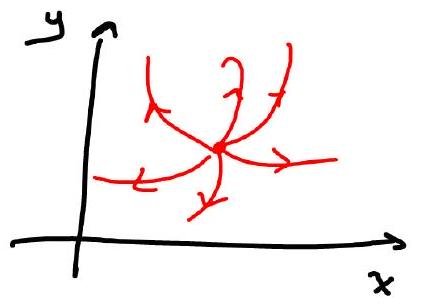
\includegraphics[width=0.5\textwidth]{2025_10_19_55a7d61d84e6ce9a1c8cg-4(2)}
\end{center}

$$
\lambda_{2}<\lambda_{1}<0
$$

stable node
\begin{center}
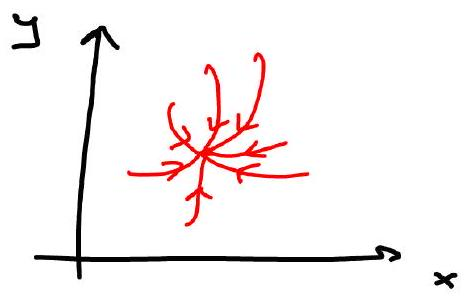
\includegraphics[width=0.5\textwidth]{2025_10_19_55a7d61d84e6ce9a1c8cg-4}
\end{center}

$$
\lambda_{2}<0<\lambda_{1}
$$

soddle node
\begin{center}
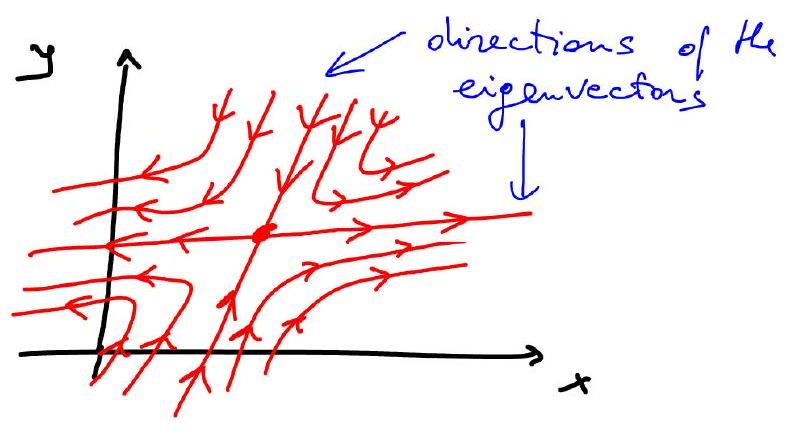
\includegraphics[width=0.5\textwidth]{2025_10_19_55a7d61d84e6ce9a1c8cg-4(3)}
\end{center}
$0<\lambda_{1}=\lambda_{2} \quad$ unstable stor

$$
\left(A=\lambda_{1} \|\right)
$$

\begin{center}
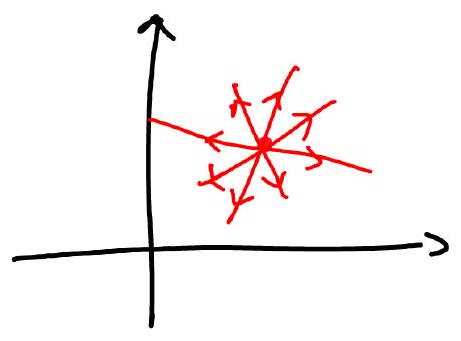
\includegraphics[width=0.5\textwidth]{2025_10_19_55a7d61d84e6ce9a1c8cg-4(1)}
\end{center}

$$
\begin{aligned}
& \lambda_{2}=\lambda_{1}<0 \quad \text { stoble stor } \\& (A=\lambda, 1)
\end{aligned}
$$

\begin{center}
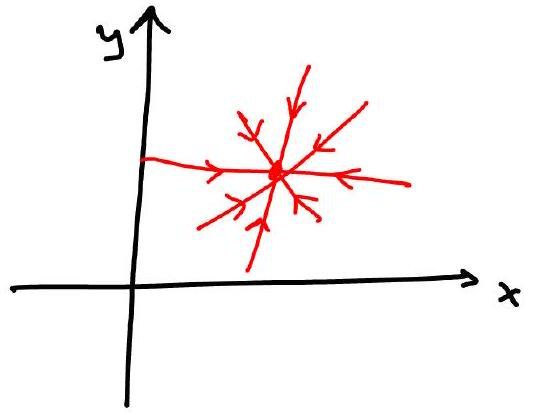
\includegraphics[width=0.5\textwidth]{2025_10_19_55a7d61d84e6ce9a1c8cg-5(1)}
\end{center}

If $A \neq \lambda_{1} \|$, then one gets degenerate (m)stable modes.
Complex eigenvolves

$$
\lambda_{1,2}=\gamma \pm i \omega
$$

$\\gamma<0 \quad$ stable focus

\begin{center}
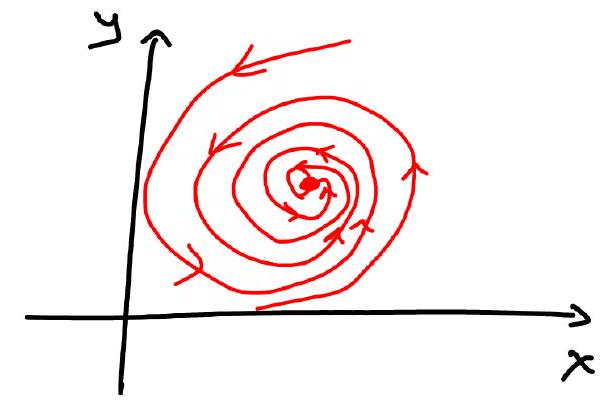
\includegraphics[width=0.5\textwidth]{2025_10_19_55a7d61d84e6ce9a1c8cg-5(3)}
\end{center}
\begin{center}
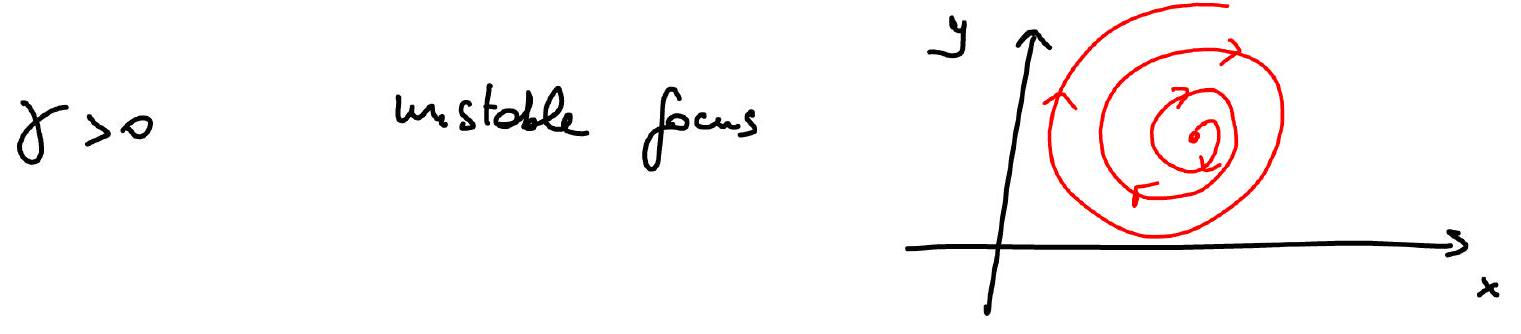
\includegraphics[width=0.5\textwidth]{2025_10_19_55a7d61d84e6ce9a1c8cg-5(4)}
\end{center}

All the above fixed points are hyperbalic. Here are a few examples of non-hyperbalic fixed points:

$$
\begin{array}{lll}
\lambda_{1}=0 & \lambda_{2}>0 & \text { line of } \\
& \left(\lambda_{1}<0\right) & \text { fixed point }
\end{array}
$$

\begin{center}
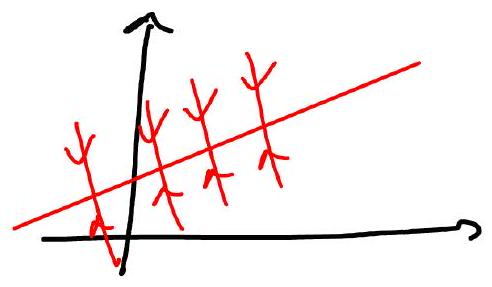
\includegraphics[width=0.5\textwidth]{2025_10_19_55a7d61d84e6ce9a1c8cg-5}
\end{center}

$$
\gamma=0 \quad \lambda_{2}= \pm i \omega
$$

\section*{center}
\begin{center}
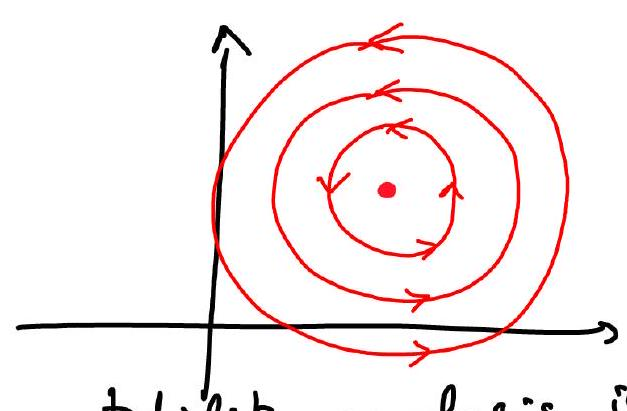
\includegraphics[width=0.5\textwidth]{2025_10_19_55a7d61d84e6ce9a1c8cg-5(2)}
\end{center}

On these latter cases the linear stobility anlysis is not sufficient to determine whether a fixed point is stable or not.

\section*{Exerciges}
\begin{enumerate}
  	item Find the fixed points of $\left\{\begin{array}{l}\\dot{x}=-x+x^{3} \\ \dot{y}=-2 y\end{array}\right.$ and classify them.
  	item Show that the linearization of the system
\end{enumerate}

$$
\left\{\begin{array}{l}
\dot{x}=-y+a x\left(x^{2}+y^{2}\right) \\dot{y}=x+a y\left(x^{2}+y^{2}\right)
\end{array}\right.
$$

incorrectly predicts that the origin is a center for all values of $a$. Indeed, the origin is a stable spinal if $a<0$, and unstable pinal if $a>0$.
[hint: to analize the nomlineer system, use polor coord. $x=r \cos \theta, y=r \sin \theta$ and find the equations for $r$ and $\theta$. Then interpret the non-lim. System.]
3) The equation of motion of a porticle is $\\ddot{x}=x-x^{3}$. Find the fixed points and classify flem. Show that the function $E=\\frac{\\dot{x}^{2}}{2}-\\frac{x^{2}}{2}+\\frac{x^{4}}{4}$ (the energy) is conserved by the dynamics and that the trajectories are clased curves difined by the contours of $E$. Draw the phase pertrait.
4) Study the system of $O D E S$ :

$$
\begin{array}{ll}
\dot{x}=x(3-x-2 y) & x, y \geqslant 0 \\dot{y}=y(2-x-y) &
\end{array}
$$

Find the fixed points and classify them. Show that the phose portroit is
\begin{center}
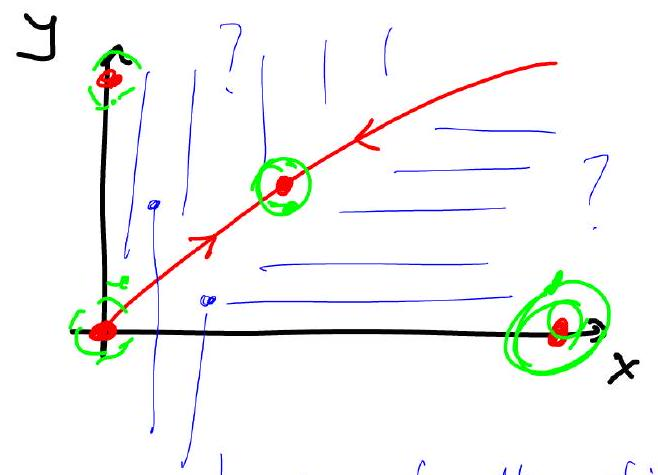
\includegraphics[width=0.5\textwidth]{2025_10_19_55a7d61d84e6ce9a1c8cg-7}
\end{center}
\basin of attraction: the set of all initial conditions which end up in one fixed point as $t \rightarrow \infty$ )

\section*{PROPERTIES OF DIFFUSION}
A first simple derivation
Let us consider a larg and thin tube filled with weter. At time $t=0$ we inject a unit amount of ink at $x=0$

Brownion mostion of pentides

$$
\begin{gathered}
 t=0, x=0 \quad V(x, t)=\text { sumal } \\W(x, t)=\frac{\# \text { of porticles in } V(x, t)}{V(x, t)}
\end{gathered}
$$
$W(x, t)$ is the density of "ink" (or Brownion) particles at position $x \in \mathbb{R}$, time $t \geqslant 0$ as the valume $V \rightarrow 0$ and the number of particle $ightarrow \infty$.
$\\int_{A} W(x, t) d x:=\text { prob. to find a porticle in the rigion } A \subseteq \mathbb{R}$. assuming that $\\int_{-\infty}^{+\infty} w(x, t) d x=1$.